\titlepageframe % Specific command 

\begin{frame}
	\frametitle{Outline}
	\tableofcontents
\end{frame}

\section{Section 1}
	\subsection{Subsection 1.1}
		\begin{tframe}{Subsection 1.1}
			\begin{itemize}
			    \item{first point}
			    \item{second point}
			    \item{third point}
			\end{itemize}
		\end{tframe}
	\subsection{Subsection 1.2}
		\begin{tframe}{Subsection 1.2}
			\begin{itemize}
				\item first point
				\item second point
				\item more points
			\end{itemize}
		\end{tframe}

\section{Section 2}
	\subsection{Subsection 2.1}
		\begin{tframe}{Subsection 2.1}
			\begin{itemize}
				\item{item 1}
				\item{item 2}
				\item{more items}
			\end{itemize}
		\end{tframe}
	\subsection{Subsection 2.2}
		\begin{tframe}{Subsection 2.2}
			\begin{center}
				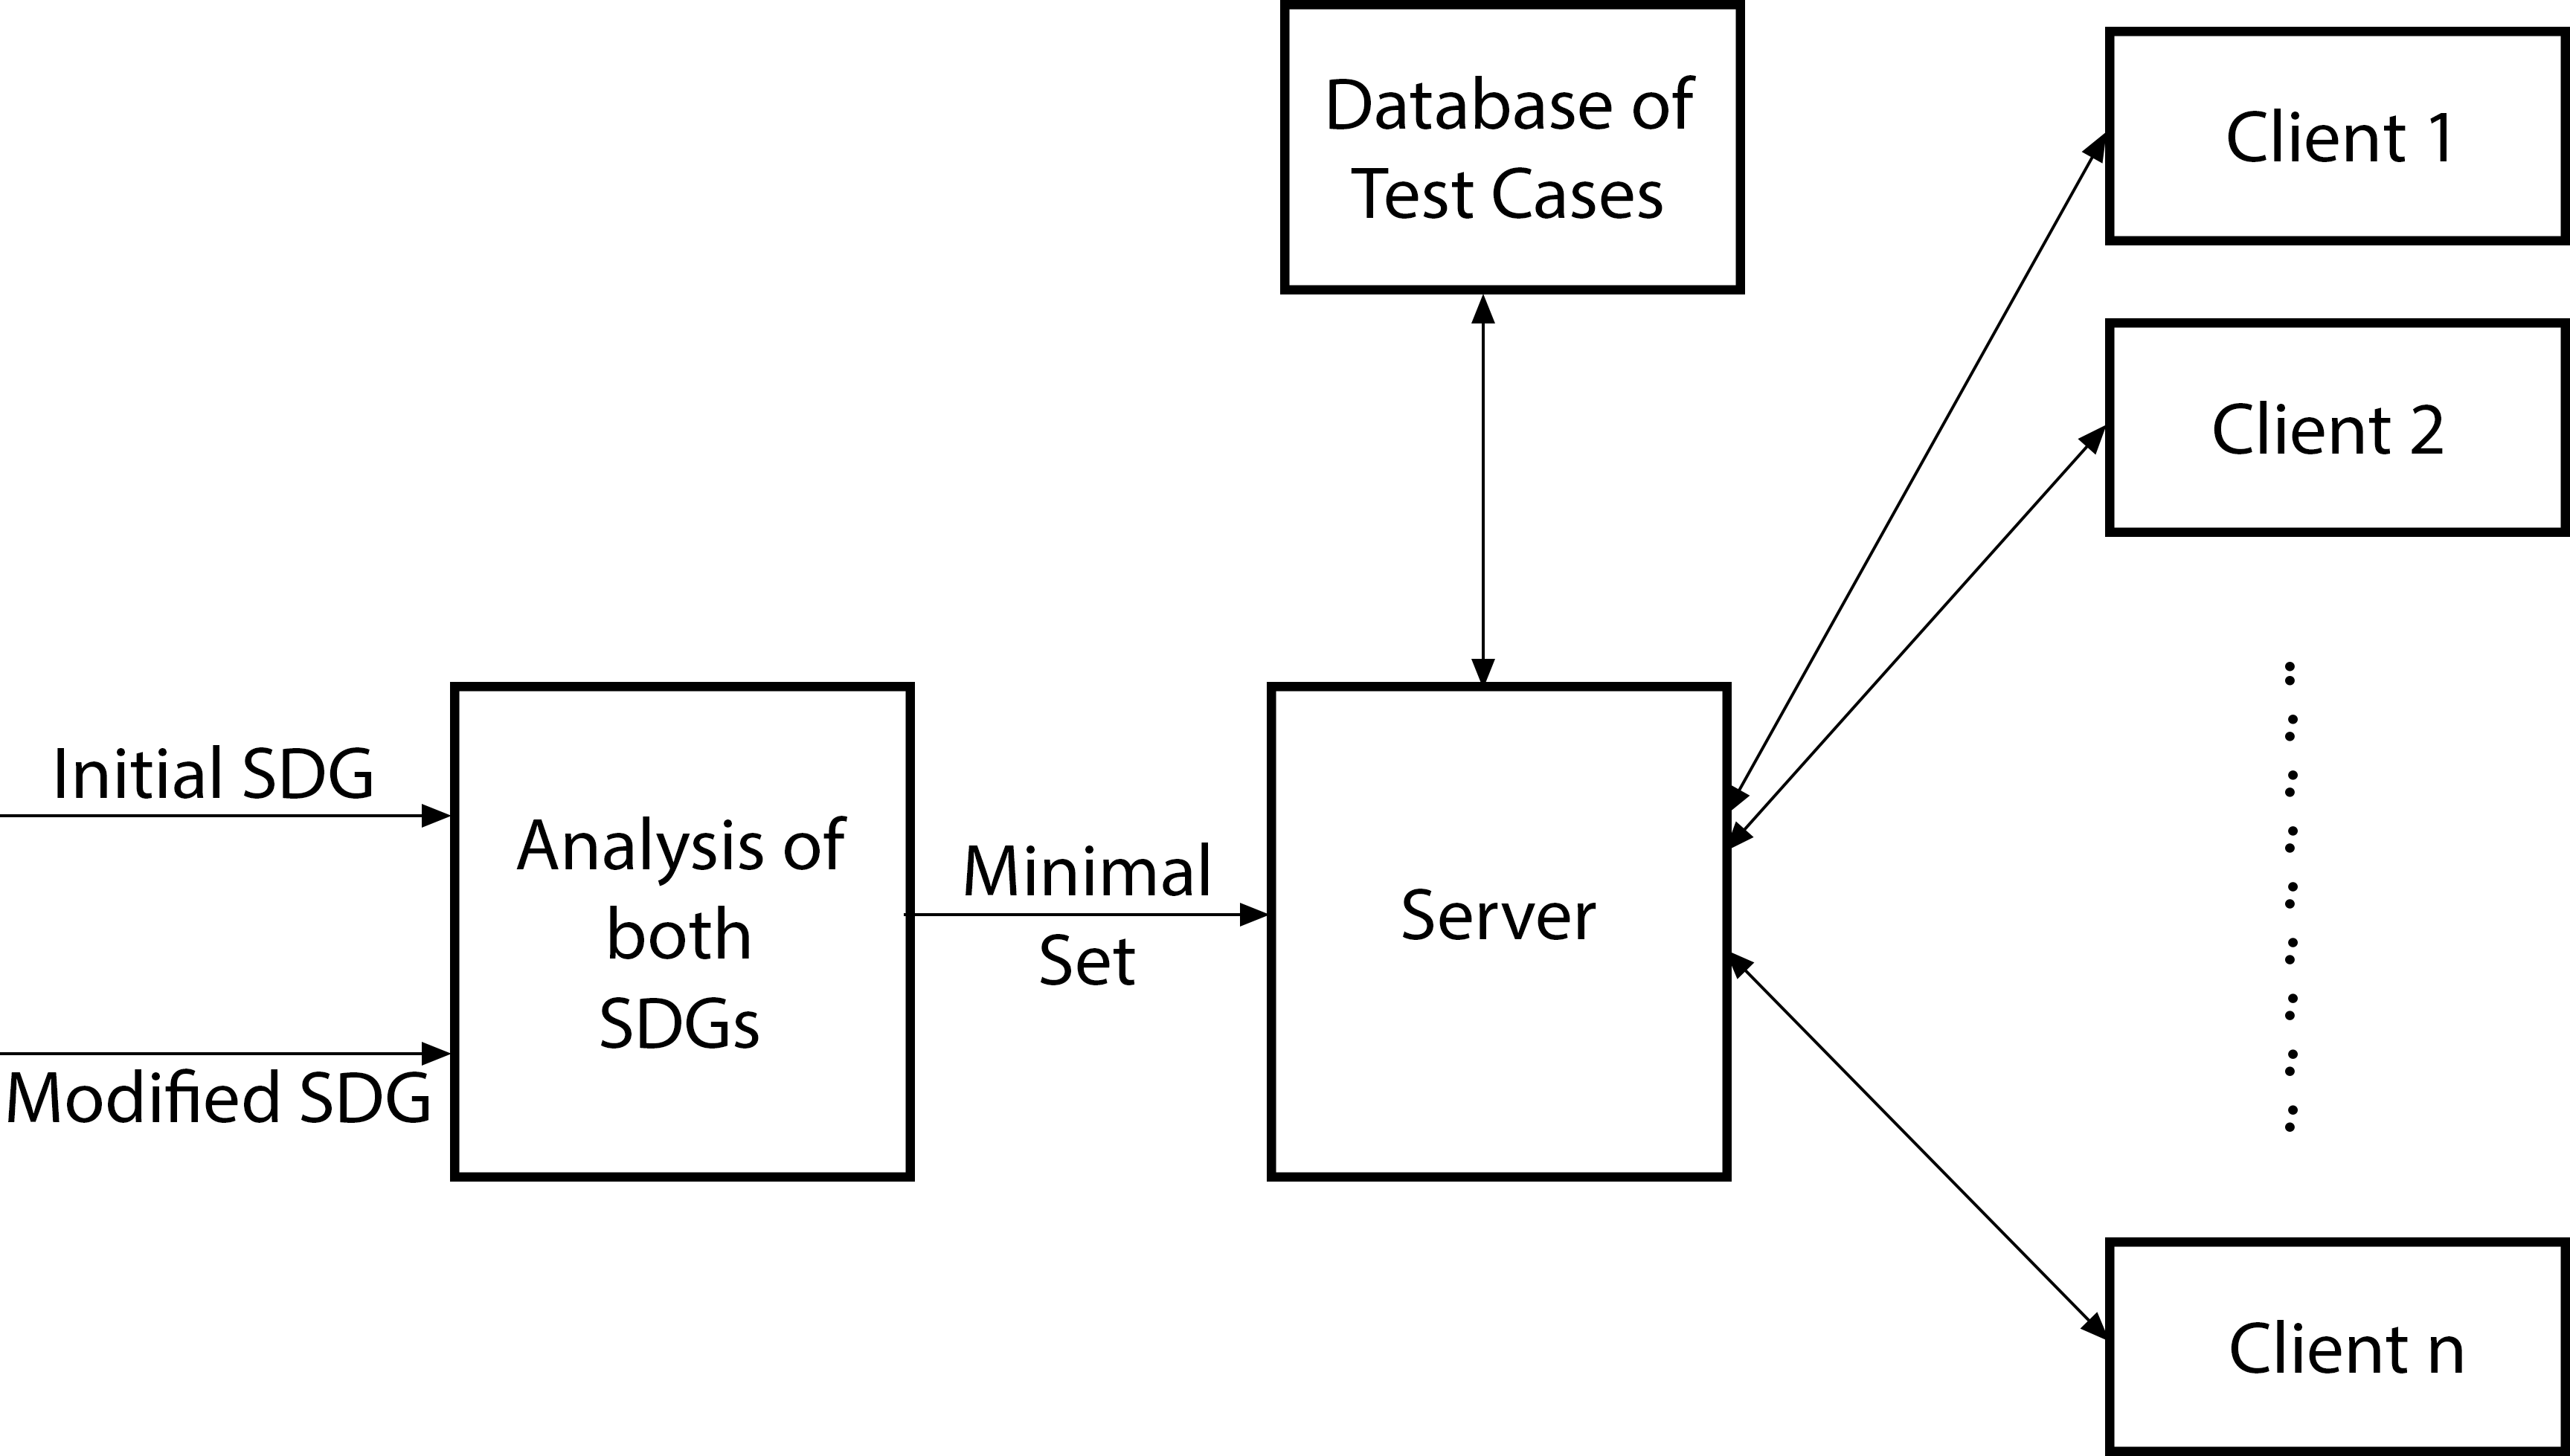
\includegraphics[scale=0.35]{Diagrams/da.png}
			\end{center}
		\end{tframe}
	\subsection{Subsection 2.3}
		\begin{tframe}{Subsection 2.3}
			\begin{itemize}
				\item Main point
				\begin{itemize}
					\item subpoint 1
					\item subpoint 2
					\item subpoint 3
					\item subpoint 4
				\end{itemize}
			\end{itemize}
		\end{tframe}
		
		\begin{tframe}{Example}
             \begin{block}{Sample Code}
						{\footnotesize
C1: public class mmseq1 \{\\
M1:	\ \ public static void main(String[ ] args) \{\\
S1:	\ \ \ \ 	int o = 0;\\
S2:	\ \ \ \ 	mathOperations mo = new mathOperations();\\
S3:	\ \ \ \ 	stringOperations so = new stringOperations();\\
S4:	\ \ \ \ 	Stack$<$Integer$>$ st = new Stack$<$Integer$>$();\\
S5:	\ \ \ \ 	String input = null;\\
S6:	\ \ \ \ 	System.out.println("Enter Options 1 to 4");\\
S7:	\ \ \ \ 	InputStreamReader ir = new InputStreamReader(System.in);\\
S8:	\ \ \ \ 	BufferedReader bR = new BufferedReader(ir);\\
S9: \	\ \ \ 	input = bR.readLine();\\
S10:	\ \ \ 	o = Integer.parseInt(input);\\
S11:	\ \ \ 	if(o ==1)\{
 }
             \end{block}
		\end{tframe}
